MongoDB ist ein in C++ geschriebenes, dokumentenorientiertes NoSQL-Datenbanksystem, das im Jahre 2009 von den Entwicklern Horowitz und Merriman als Open-Source Datenbank veröffentlicht wurde und die am weitest-verbreiteste NoSQL-Datenbank. (Stand April 2021) [MongoDB1.7] Die Intention der Gründer war es, eine Datenbank mit höherer Skalierbarkeit, Flexibilät und Performance zu entwerfen, die auf auf einer einfachen Handhabung beruht. [MongoDB1.65]
\newline

Gründe der Popularität der Datenbank ist neben den oben erwähnten Eigenschaften die flexible Gestaltungsmöglichkeit der Datenstrukturen sowie die Unterstützung durch zahlreiche Programmiersprachen und Betriebssysteme.
\newline

Dem Konzept des CAP-Theorems folgend steht MongoDB für Konsistenz und Partitionstoleranz, dafür ordnet sich die Verfügbarkeit den anderen Eigenschaften unter.
\newline

\textbf{2.2.4.3 Aufbau/Struktur}
\newline
\textbf{2.2.4.3 Dokumente}
\newline
Während MongoDB für Datenaustausch das JSON-Format nutzt, hält es seine Dokumente im Binary JSON-Format (BSON), einer binärcodiertem Erweiterung des JSON-Formats. Daten im BSON-Format enthalten zusätzlich Informationen zum Typ und zur Länge der Informationen, wodurch schnelleres Parsen von Daten möglich ist. Des Weiteren werden ist BSON um zusätzliche Datentypen wie 32- und 64-bit Integer oder das Datum erweitert. [MongoDb1.8 https://www.mongodb.com/json-and-bson] 
\newline

\begin{figure}[h]
\centering
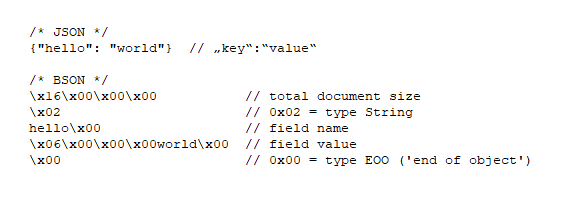
\includegraphics[]{images/BSON.PNG}
\caption{Graphikdatenbank Beispiel [NoSql 1.2]}
\end{figure}



\textbf{CRUD}
\newline
Im Vergleich zu relationalen Datenbanken benutzt MongoDB keine Abfragesprache wie SQL, sondern 


Wired Tiger?
Storage Engine
Replica Sets
Oplog
Sharding
\newline

\textbf{Technische Grundlagen}
/
Replica
Transaktionen
\newline

\textbf{Verwaltungswerkzeuge}
Mongo Shell
Treiber
Grafische Oberflächen
